\documentclass{article}
\usepackage[cm]{fullpage}
\usepackage{layout}
\usepackage{hyperref}   % For links
\usepackage{array}      % For tables
\usepackage{graphicx} % Required for inserting images
\usepackage{xcolor}
\usepackage[dvipsnames]{xcolor}
\usepackage{listings}   % For coding
\usepackage{amssymb}    % For square
\usepackage{amsmath}    % For cases


\title{Teoremas, Proposiciones y Corolarios}
\author{Bander}
\date{Julio 2025}

\begin{document}
%\layout para ver el layout actual
\maketitle

\begin{flushleft}
  Este es un resumen de los teoremas en mis palabras y con sobreexplicación seguramente para así 
  yo lo entiendo. 

  No pretendo reemplazar la documentación oficial, si no que es para tener una explicación para 
  mi yo del futuro.
\end{flushleft}

\pagebreak

\begin{flushleft}
  \textbf{Proposición 1:} 
  \textit{Sea $f : \{0,1\}^* \rightarrow \{0,1\}^*$, sea T una función construible en
  tiempo y sea $\Gamma$ un alfabeto. Si f es computable en tiempo $T(n)$ por una máquina $M = 
  (\Gamma, Q, \delta)$, entonces f es computable en tiempo $O(log|\Gamma| \cdot T(n))$ por 
  una máquina $M' = (\Sigma, Q', \delta')$ donde $\Sigma = \{0,1,\triangleright, \square \}$
  es el alfabeto estándar.}\\[0.5em]

  \textbf{\textcolor{Mulberry}{Demostración:}} \\[0.5em]

  $|\Gamma|$ es la cantidad de estados que hay originalmente, para codificar cada estado de $Q$
  en $Q'$ se usa el alfabeto $\Sigma$ (binario), por lo cual conlleva $log_2|\Gamma|$ bits por
  estado (por convencion usamos que $log_2|\Gamma| = log|\Gamma|$ bits).\footnote{La base  no importa en la notación big $O$ para los logarítmos ya que difieren entre
  si por una constante multiplicativa debido a cómo se puede cambiar la base de un logarítmo 
  $(log_b n = \frac{log_k n}{log_k b})$}

  Eso se traslada a $\delta'$  también, por lo cual, lo que antes llevaba un símbolo perteneciente a 
  $\Gamma$ ahora lleva $log_2|\Gamma|$ símbolos de $\Sigma$ (pej.: $A = 1010$).
\end{flushleft}

\begin{flushleft}
  \textbf{\hypertarget{prop2}{Proposición 2:}} 
  \textit{Sea $f : \{0,1\}^* \rightarrow \{0,1\}^*$ y sea $T$ una función construible en tiempo. 
  Si $f$ es computable en tiempo $T(n)$ por una máquina estándar de $k \geq 3$ cintas (entrada, 
  salida y $k - 2$ cintas de trabajo), entonces $f$ es computable en tiempo $O(T(n)^2)$ por una 
  máquina de cinta única.}\\[0.5em]

  \textbf{\textcolor{Mulberry}{Demostración:}} \\[0.5em]

  Puedo alternar los símbolos de las $k$ cintas en la cinta única y usar símbolos característicos
  para indicar dónde está la cabeza de cada cinta.

  En la posición $i$ está el caracter $\lceil \frac{i}{k} \rceil$ de la cinta $i$ mod $k$.

  \begin{figure}[h] 
    \centering 
    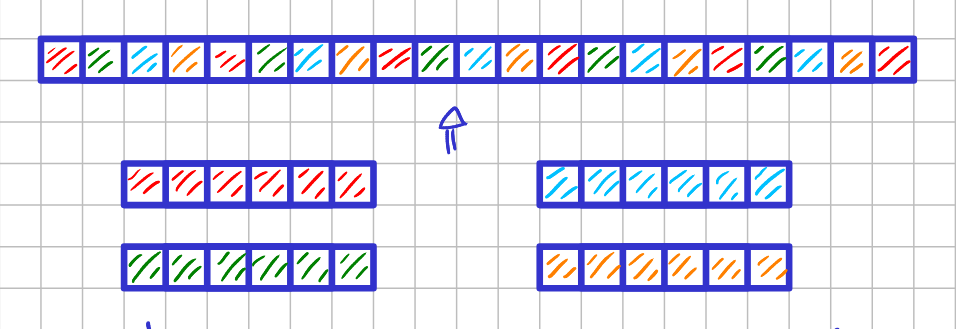
\includegraphics[width=10cm, height=4cm]{./imagenes/4_cintas_a_1.png}
  \end{figure}

  Queda en $O(T(n)^2)$ debido a que por cada paso de $\delta$ debo primero ubicar cada cabeza para 
  ver que accionar y después modificar cada cabeza como lo indique $\delta$. O sea, por cada paso 
  recorro toda la cinta 2 veces.
\end{flushleft}

\begin{flushleft}
  \textbf{Proposición 3:}
  \textit{Sea $f : \{0,1\}^* \rightarrow \{0,1\}^*$ y sea $T$ una función construible en tiempo. Si $f$
  es computable en tiempo $T(n)$ por una máquina estándar, entonces hay una máquina oblivious que 
  computa $f$ en tiempo $O(T(n)^2)$.}\\[0.5em]

  \textbf{\textcolor{Mulberry}{Demostración:}} \\[0.5em]

  La máquina obliviousse mueve un patrón fijo en cada paso (barre toda la cinta) y cambia la cinta según 
  los cambios que se piden. Es muy similar a la \hyperlink{prop2}{\textcolor{Rhodamine}{proposición 2}}.
\end{flushleft}

\begin{flushleft}
  \textbf{Proposición 4:}

  \textit{Sea $f : \{0,1\}^* \rightarrow \{0,1\}^*$ y $T$ una función construible en tiempo. Si $f$
  es computable por una máquina con cintas bi-infnitas en tiempo $T(n)$, entonces $f$ es computable
  por una máquina estándar en tiempo $O(T(n))$}\\[0.5em]

  \textbf{\textcolor{Mulberry}{Demostración:}} \\[0.5em]

  Se puede doblar la cinta bi-infinita de manera que rebota en el símbolo $\triangleright$ para 
  ver ambos infinitos.

  \begin{figure}[h] 
    \centering 
    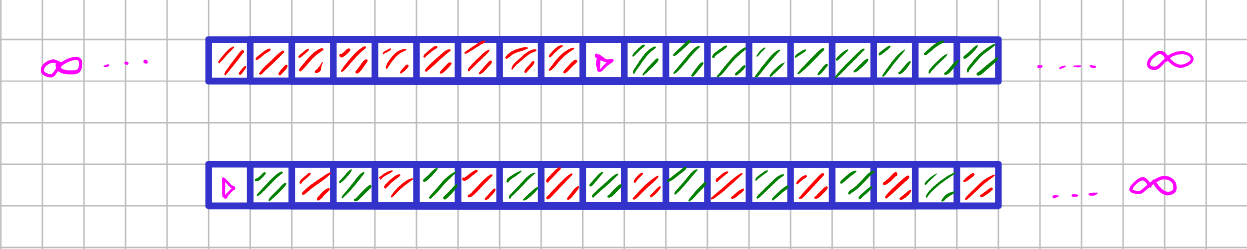
\includegraphics[width=13cm, height=3cm]{./imagenes/biinfinita_a_infinita.png}
  \end{figure}
\end{flushleft}

\pagebreak

\begin{flushleft}
  \textbf{Teorema 1:}
  \textit{[Turing 1936] halt no es computable.}\\[0.5em]

  \textbf{\textcolor{OliveGreen}{Recordatorio:}}

  \[
    halt(x) = 
    \begin{cases}
    1 & \text{si la máquina con entrada } x \text{ termina } (M_x(x)) \\
    0 & \text{si no}
    \end{cases}
  \]

  \textbf{\textcolor{Mulberry}{Demostración:}} \\[0.5em]

  Sale por diagonalización. Tengo que:
  
  \[
    \begin{array}{c|cccc}
    & M_1 & M_2 & M_3 & \cdots \\
    \hline
    1 & M_1(1) &  &  & \\
    2 &  & M_2(2) &  & \\
    3 &  &  & M_3(3) & \\
    \vdots &  &  &  & \ddots \\
    \end{array}
  \]

  Defino entonces $M$ tal que $M(x)$ termina sii $halt(x) = 0$.

  $M(\langle M \rangle)$ termina $\iff$ $halt(\langle M \rangle) = 0$ $ \iff M(\langle M \rangle)$ 
  no termina. \textcolor{Red}{Absurdo!}
\end{flushleft}

\begin{flushleft}
  \textbf{\hypertarget{teo2}{Teorema 2:}}
  \textit{Existe una máquina U que computa la función $u(\langle i,x \rangle) = M_i(x)$. Más aún, 
  si $M_i$ con entrada $x$ termina en $t$ pasos, entonces $U$ con entrada $\langle i,x \rangle$ termina
  en $c \cdot t \cdot  log(t)$ pasos, donde $c$ depende solo de $i$.}\\[0.5em]

  \textbf{\textcolor{Mulberry}{Demostración:}} \\[0.5em]

  Pone en cada cinta de trabajo la simulación de la máquina estándar de $M$. O sea, en 
  
  \begin{itemize}
    \item $\#1$: La entrada $x$.
    \item $\#2$: Cinta de trbajo de $M$.
    \item $\#3$: Estado de $M$.
  \end{itemize}

  Si $\#3 = [q_f]$ termina la ejecución $M$.

  Por cada paso de M busco $\delta$ en la entrada de la máquina $U$.

  \begin{figure}[h] 
    \centering 
    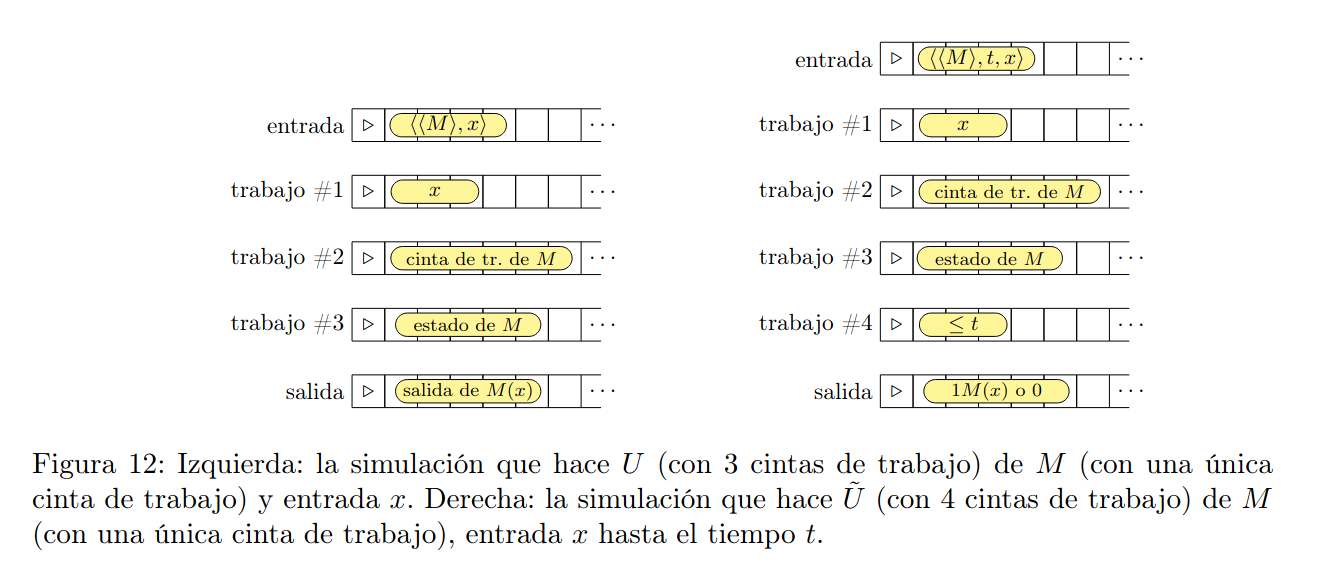
\includegraphics[width=17cm, height=7cm]{./imagenes/simulacion_con_maq_universal.png}
  \end{figure}
\end{flushleft}

\begin{flushleft}
  \textbf{Teorema 3:}
  \textit{Existe una máquina $\widetilde{U}$ que computa la función $\widetilde{u}(\langle i,t,x \rangle)$
  en tiempo $c \cdot t \cdot log(t)$, donde $c$ depende solo de $i$.} \\[0.5em]

  \textbf{\textcolor{Mulberry}{Demostración:}} \\[0.5em]

  Es muy similar al \hyperlink{teo2}{\textcolor{Rhodamine}{teorema 2}} pero con una cinta más de trabajo
  para llevar registro de $i$ (cantidad de pasos en la simulación).
\end{flushleft}

\pagebreak

\begin{flushleft}
  \textbf{Teorema 4:}
  $\mathsf{P} \subseteq \mathsf{NP}$ \\[0.5em]

  \textbf{\textcolor{Mulberry}{Demostración:}} \\[0.5em]

  Sea $\mathcal{L} \in \mathsf{P}$. $\mathcal{L}(M)$, con $M$ una máq. det. que corre en tiempo 
  polinomial.

  Tomás el polinomio $p$ de la definición como $p(|x|) = 0$. Defino $M'$ det. y que corre en tiempo poly.
  y el certificado $c = \varepsilon$ (donde $\varepsilon$ es la cadena vacía), entonces tengo que $M'$ con 
  entrada $\langle x,c \rangle$ copia el comportamiento de $M$ con entrada $x$.
\end{flushleft}

\begin{center}
  $x \in \mathcal{L} \iff M(x) = 1$  \\
  $\iff M'(\langle x,c \rangle) = 1$  \\
  $\iff \exists c. c\in \{0,1\}^0$ tal que $M'(\langle x,c \rangle)$ (Definición de $\mathsf{NP}$)
\end{center}

\begin{flushleft}
  \textbf{Teorema 5:}
  $\mathsf{NP} = \bigcup_{c \in \mathbb{N}} \mathsf{NDTime}(n^c)$ \\[0.5 em]

  \textbf{\textcolor{Mulberry}{Demostración:}} \\[0.5em]

  \textcolor{Mulberry}{$\bigcup_{c \in \mathbb{N}} \mathsf{NDTime}(n^c) \subseteq \mathsf{NP}$:}

  Sea $\mathcal{L} \in \bigcup_{c \in \mathbb{N}} \mathsf{NDTime}(n^c)$ quiero ver que $\mathcal{L} \in 
  \mathsf{NP}$.
  Sea $N$ una máq. no-det. y $p$ un polinomio tal que $N$ corre en tiempo $p(n)$ y $\mathcal{L}(N)$.

  Existe una máq. det. $M$ tal que $M$ con entrada $\langle x,u \rangle$ verifica que $u$ sea la 
  codifcación del cómputo aceptador de $N$ a partir de $x$. 
  $M$ simula $N$ con entrada $x$ paso a paso, y en cada iteración $i$ usa la primera o la segunda 
  componente de $\delta$ según el valor de $u(i)$ para saber qué hacer.

  Luego, $x \in \mathcal{L} \iff \exists u$ . $u \in  \{ 0,1 \}^{p(|x|)}$ tal que $M(\langle x,u \rangle)
  = 1$. Como $M$ corre en tiempo polinomial (ya que es solo recorrer las decisiones en $N$ con $u$), 
  concluímos que $\mathcal{L} \in \mathsf{NP}$.\\[0.5em]

  \textcolor{Mulberry}{$\mathsf{NP} \subseteq \bigcup_{c \in \mathbb{N}} \mathsf{NDTime}(n^c)$:}

  Sea $\mathcal{L} \in \mathsf{NP}$ quiero ver que $\mathcal{L} \in \bigcup_{c \in \mathbb{N}} 
  \mathsf{NDTime}(n^c)$. Para esto uso la máq. $M$ det. que corre en tiempo poly de la definición y la 
  simulo con una no-det. que hace lo mismo pero inventando el certificado $u$ por lo que te queda que corre
  en tiempo poly al ser que $M$ corría en tiempo poly.
\end{flushleft}

\begin{flushleft}
  \textbf{Teorema 6:}
  \textit{Existe una máquina no-determinística $NU$ tal que $NU$ acepta $(\langle i,x \rangle)$ sii $N_i$
  acepta $x$ y si $N_i$ corre en tiempo $T(n)$ entonces $NU(\langle i,x \rangle)$ decide si $N_i$ acepta o 
  rechaza $x$ en $c \cdot T(|x|)$ pasos, donde $c$ depende solo de $i$.} \\[0.5em]

  \textbf{\textcolor{Mulberry}{Demostración:}} \\[0.5em]

  Similar al \hyperlink{teo2}{\textcolor{Rhodamine}{teorema 2}}. No tiene el logarítmo porque puede 
  adivinar no deterministamente la secuencia de elecciones que  seguiría $N_i$ para aceptar $x$.
\end{flushleft}

\begin{flushleft}
  \textbf{Teorema 7:}
  \textit{La relación $\leq_p$ es transitiva.} \\[0.5em]

  \textbf{\textcolor{Mulberry}{Demostración:}} \\[0.5em]

  Sea $\mathcal{L} \leq_p \mathcal{L'}$ vía $g$ quiero ver que $\mathcal{L} \leq_p \mathcal{L''}$.
\end{flushleft}
\begin{center}
  $x \in \mathcal{L} \iff f(x) \in \mathcal{L'} \iff g(f(x)) \in \mathcal{L''}$
\end{center}
\begin{flushleft}
  Ahora quiero ver que $g \circ f$ es computable en tiempo polinomial respecto $|x|$.

  Sea $M_f$, $M_g$ tal que $M_f$ computa $f$ en tiempo poly y $M_g$ computa $g$ en tiempo poly. \\[0.5em]
  $M_{g \circ f} : \langle x \rangle $

  \quad $y := M_f(x)$ \qquad \textcolor{OliveGreen}{$O(n^c)$ A lo sumo su salida es polinomial respecto $n$ 
  ($n = |x|$)} 

  \quad return  $M_g(y)$ \qquad \textcolor{OliveGreen}{$O((n^c)^d) = O(n^{cd})$ A lo sumo es poly respecto a 
  $|y|$}
\end{flushleft}

\begin{flushleft}
  \textbf{\hypertarget{teo8}{Teorema 8:}}
  \textit{Si }$\mathsf{NP}$-hard $\cap \ \mathsf{P} \neq \emptyset$\textit{, entonces} $\mathsf{P} = 
  \mathsf{NP}$. \\[0.5 em]

  \textbf{\textcolor{Mulberry}{Demostración:}} \\[0.5em]

  Si $\mathcal{L} \in \mathsf{NP}$-hard $\cap \ \mathsf{P}$, entonces puedo tomar cualquier $\mathcal{L'} \in
  \mathsf{NP}$ y reducirlo a $\mathcal{L}$, por lo cuál tengo una $f$ computable poly tal que:
\end{flushleft}
\begin{center}
  $x \in \mathcal{L'} \iff f(x) \in \mathcal{L}$
\end{center}
\begin{flushleft}
  Entonces a la $\mathcal{L'}(M_{\mathcal{L'}})$ la declaro como: \\[0.5em]
  
  $M_{\mathcal{L'}}: \langle x \rangle$
  
  \quad $y := M_f(x)$ \qquad \textcolor{OliveGreen}{$O(n^c)$}

  \quad $M_{\mathcal{L}}(y)$ \qquad \textcolor{OliveGreen}{$O(n^{cd})$} \\[0.5em]

  $M_{\mathcal{L'}}$ es entonces una máq. det. que corre en tiempo poly por lo que $\mathcal{L'} \in 
  \mathsf{P}$. O sea $\mathsf{P} = \mathsf{NP}$, al ser que $\mathcal{L'}$ es genérico.
\end{flushleft}

\pagebreak

\begin{flushleft}
  \textbf{Teorema 9:}
  \textit{Si }$\mathcal{L} \in \mathsf{NP}$-completo\textit{, entonces} $\mathcal{L} \in \mathsf{P} \iff 
  \mathsf{P} = \mathsf{NP}$. \\[0.5em]

  \textbf{\textcolor{Mulberry}{Demostración:}} \\[0.5em]

  \textcolor{Mulberry}{$\mathcal{L} \in \mathsf{P} \Rightarrow \mathsf{P} = \mathsf{NP}$:}

  Si $\mathcal{L}$ es $\mathsf{NP}$-completo y a su vez $\mathcal{L} \in \mathsf{P}$, lo único que agrega 
  que $\mathcal{L} \in \mathsf{NP}$-completo es que $\mathcal{L} \in \mathsf{NP}$-hard.\footnote{
  $\mathcal{L}$ ya era $\mathsf{NP}$, porque $\mathsf{P} \subseteq \mathsf{NP}$}

  Luego, por el \hyperlink{teo8}{\textcolor{Rhodamine}{teorema 8}} obtengo que $\mathsf{P} = \mathsf{NP}$.
  \\[0.5em]

  \textcolor{Mulberry}{$\mathsf{P} = \mathsf{NP} \Rightarrow \mathcal{L} \in \mathsf{P}$:}

  Si $\mathsf{P} = \mathsf{NP}$, entonces todos los problemas de $\mathsf{NP}$ se pueden resolver en tiempo
  poly, en particular también todos los $\mathsf{NP}$-completos.
\end{flushleft}

\begin{flushleft}
  \textbf{Proposición 6:}
  $\mathsf{TMSAT} \in \mathsf{NP}$-completo.

  
\end{flushleft}
\end{document}
